\chapter{Модельные каскады для разделения бинарных смесей.}


Трудности решения (\ref{GrindEQ__1_24_})--(\ref{GrindEQ__1_27_}), (\ref{GrindEQ__1_35_})--(\ref{GrindEQ__1_38_}) и (\ref{GrindEQ__1_39_})--(\ref{GrindEQ__1_40_}) в общем случае, стимулировали развитие упрощенных подходов, которые позволяют получить аналитическое решение для данных систем при введении определенных предположений. Полученные в результате таких упрощений физико-математические модели симметрично-противоточного каскада сохраняют закономерности молекулярно-селективного массопереноса, но позволяют заметно упростить соответствующие расчетные процедуры для определения оптимальных параметров каскада. Такие каскады получили название модельных \cite{minenkoTeoriiKaskadovDlya1965, delagarzaMulticomponentIsotopeSeparation1961, zhigalovskiyLekcionnyeMaterialyPo1999, kolokoltsovDesignCascadesSeparating1970, kolokolcovVoprosuPostroeniiKaskadov1970, minenkoPredelnoeObogashcheniePromezhutochnyh1972, yamamotoMulticomponentIsotopeSeparating1978, wuStudyMulticomponentIsotope, borisevichRascheteKaskadovDopolnitelnym1993, woodCriterionEffiencyMultiisotope1999, sulaberidzeOsobennostiObogashcheniyaKomponentov2006, sazykinKvaziidealnyeKaskadyDlya2000, sulaberidzeSravnenieOptimalnyhModelnyh2008}.

Модельные каскады действуют как физически эквивалентные представления и, как показано в \cite{sulaberidzeClassificationModelCascades2020}, могут быть выведены из <<обобщенного модельного каскада>>, которым является симметрично-противоточный каскад с постоянными по его длине относительными коэффициентами разделения).

Целесообразной областью применения теории модельных каскадов является ее использование при предварительном рассмотрении актуальных проблем современной теории разделения многокомпонентных изотопных смесей в каскадах и смежных с разделительной наукой областей, таких, например, как ядерная энергетика.
% В рамках данной работы анализ строится на основе теории модельных каскадов, однако выявленные физические закономерности массопереноса в рассмотренных каскадных схемах справедливы и в близких к реализуемых в производственных условиях прямоугольных и прямоугольно секционированных каскадов.

Далее рассмотрим подробнее математические модели, нашедшие свое применение в расчетных исследованиях.


\section{«Идеальный» каскад}

\subsection{«Идеальный» каскад для разделения бинарных смесей как частный случай симметрично-противоточного каскада с постоянными коэффициентами разделения.}

Условие \ref{GrindEQ__1_94_} позволяет однозначно определить распределение потоков в идеальном каскаде. Перепишем условие \ref{GrindEQ__1_94_} в виде двух равенств:
\begin{equation} \label{GrindEQ__1_100_} 
\delta '_{S-1} =\Delta _{S-1} ,\; \; \Delta _{S} =\delta ''_{S+1} .~~~                         ~ 
\end{equation} 

или, в первом из них, смещая индексы и используя  в виде единого соотношения, получим
\begin{equation} \label{GrindEQ__1_101_} 
\delta '_{S} =\Delta _{S} =\delta ''_{S+1} .~~~~~~~~~~~            ~~~~~~~~~~~~~~~~ 
\end{equation} 

Подставляя \ref{GrindEQ__1_101_} в \ref{GrindEQ__1_80_} и обозначая поток в идеальном каскаде через $L_{S}^{*} ,$ получим
\begin{equation} \label{GrindEQ__1_102_} 
\begin{array}{l} {L_{S}^{*} =\frac{P(c_{P} -c_{S} )}{\theta _{S} \delta '_{S} } ,} \\ {\; \; \; \; \; s=f,\; f+1,\; ...,\; N-1,} \end{array} 
\end{equation} 
\begin{equation} \label{GrindEQ__1_103_} 
L_{N}^{*} =\frac{P}{\theta _{N} } .  ~~~~~              ~~~~~~~ 
\end{equation} 

Аналогично распределение потоков в обеднительной части идеального каскада можно представить в виде
\begin{equation} \label{GrindEQ__1_104_} 
L_{S}^{*} =\frac{W(c_{S} -c_{W} )}{\theta _{S} \delta '_{S} } ,~~~~~~~~~~~~~~~~~~~~        ~~~~~ 
\end{equation} 
\begin{equation} \label{GrindEQ__1_105_} 
L_{1}^{*} =\frac{W}{1-\theta _{1} } .  ~~~             ~~~~~~~~~~ 
\end{equation} 

Величина обогащения на ступени $\delta '_{S} $ определяется соотношением \ref{GrindEQ__1_9_}, а коэффициент деления потоков формулой \ref{GrindEQ__1_48_}. Таким образом, систему уравнений, позволяющую рассчитывать распределения концентраций, коэффициентов деления потоков и расходов в идеальном каскаде можно представить в виде:
\begin{equation} \label{GrindEQ__1_106_} 
\Delta _{S} =c_{S+1} -c_{S} =\frac{(\alpha _{S} -1)c_{S} (1-c_{S} )}{1+(\alpha _{S} -1)c_{S} } =\frac{\varepsilon '_{S} c_{S} (1-c_{S} )}{1+\varepsilon '_{S} c_{S} } , 
\end{equation} 
\begin{equation} \label{GrindEQ__1_107_} 
\theta _{S} =\frac{(\beta _{S} -1)\left[1+(\alpha _{S} -1)c_{S} \right]}{q_{S} -1} =\frac{\varepsilon ''_{S} (1+\varepsilon '_{S} c_{S} )}{(1-\varepsilon ''_{S} )\varepsilon _{S} } ,~              ~ 
\end{equation} 

$L_{S}^{*} =\frac{P(c_{P} -c_{S} )}{\theta _{S} \delta '_{S} } $ - для обогатительной части каскада,

\noindent $L_{S}^{*} =\frac{W(c_{S} -c_{W} )}{\theta _{S} \delta '_{S} } $ - для обеднительной части каскада,

с граничными условиями
\begin{equation} \label{GrindEQ__1_110_} 
\theta _{N} L_{N}^{*} =P,\quad c'_{N} =c_{P} ,~~~~~~~~~~~~~~~~~~~~~~~~~~~~~~ 
\end{equation} 
\begin{equation} \label{GrindEQ__1_111_} 
(1-\theta _{1} )L_{1}^{*} =W,\quad c''_{1} =c_{W} .~~~~~~~~~~~~~~~~~~~ 
\end{equation} 

Кроме того, к условиям \ref{GrindEQ__1_110_}, \ref{GrindEQ__1_111_} необходимо добавить условие несмешения концентраций на входе в ступень питания $c_{F} =c_{f} $.

Обратим внимание на тот факт, что система \ref{GrindEQ__1_106_} -- \ref{GrindEQ__1_107_} записана в конечных разностях и её следует решать "шаг за шагом".

Наиболее изученными и имеющими практическое значение являются свойства идеального каскада при малых обогащениях на отдельных ступенях (случай слабого обогащения).

\subsection{Идеальный каскад с малым обогащением на ступени (случай слабого обогащения).}

В случае слабых одинаковых обогащений на ступенях формулы \ref{GrindEQ__1_106_}-\ref{GrindEQ__1_107_} упрощаются. Тогда с учетом \ref{GrindEQ__1_82_}, \ref{GrindEQ__1_10_} - \ref{GrindEQ__1_12_} и факта, что параметры каскада от ступени к ступени изменяются непрерывно, система \ref{GrindEQ__1_106_} - \ref{GrindEQ__1_107_} приводится к виду:
\begin{equation} \label{GrindEQ__1_112_} 
\frac{dc}{ds} =\frac{1}{2} \varepsilon c(1-c), 
\end{equation} 
\begin{equation} \label{GrindEQ__1_113_} 
\theta \approx \frac{1}{2} , 
\end{equation} 
\begin{equation} \label{GrindEQ__1_114_} 
L^{*} =\frac{4P(c_{P} -c)}{\varepsilon c(1-c)}  
\end{equation} 
для обогатительной части каскада и
\begin{equation} \label{GrindEQ__1_115_} 
L^{*} =\frac{4W(c-c_{W} )}{\varepsilon c(1-c)} ,~~~                              
\end{equation} 
для обеднительной части каскада.

Из уравнения \ref{GrindEQ__1_112_} следует, что градиент концентрации в идеальном каскаде вдвое меньше, чем при безотборном режиме работы каскада.

Уравнение \ref{GrindEQ__1_112_} легко интегрируется и дает распределение $c(s)$, а уравнения \ref{GrindEQ__1_114_} и \ref{GrindEQ__1_115_} дают распределения $L^{*} (s)$, выраженные через параметр $c(s)$.  Уравнения \ref{GrindEQ__1_112_} - \ref{GrindEQ__1_115_} называют уравнениями \textit{идеального симметричного каскада}. Как видно из \ref{GrindEQ__1_112_} и \ref{GrindEQ__1_115_} потоки $L^{*} $ обратно пропорциональны $\varepsilon $. Этот факт существенен для практики. Так, для газодиффузионного метода разделения $\varepsilon {\sim 10}^{{-3}} $ [3,~7] и, следовательно, потоки (производительности) ступеней должны в тысячи раз превышать потоки отбора \textit{P} и отвала \textit{W}. Интегрирование уравнения \ref{GrindEQ__1_112_} для любого интервала концентраций $c_{1} \le c\le c_{2} $ дает соответствующее число ступеней
\begin{equation} \label{GrindEQ__1_116_} 
s_{12} =\frac{2}{\varepsilon } \ln \frac{c_{2} /1-c_{2} }{c_{1} /1-c_{1} } . ~~~~~~~~~~~~~~~~~~~~~~~~~~~~ ~~~~ 
\end{equation} 

Полагая $c_{1} $ равным $c_{W} $ или $c_{F} $ и $c_{2} $ равным $c_{F} $ или $c_{P} $ можно получить формулы для расчета числа ступеней в обеднительной и обогатительной части каскада соответственно.

\begin{figure}[ht]
    \centerfloat{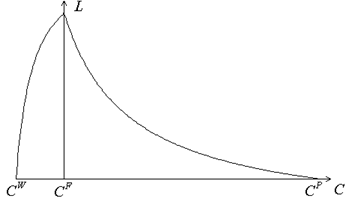
\includegraphics[scale=0.99]{img/depend.png}}
    \caption{Зависимость потока каскада от концентрации.}\label{depend}
  \end{figure}

На рис. \ref*{depend} показана зависимость потока питания ступеней от концентрации. Выбранный случай характерен для разделения изотопов урана и других элементов с низким содержанием ценного компонента $c_{F} <<1$. В секции обогащения изменение потоков (формула 1.114) имеет гиперболический характер. Потоки уменьшаются от ступени питания в сторону отбора с постоянно снижающейся скоростью. В отличие от этого в секции обеднения небольшое уменьшение вблизи ступени питания сменяется резким спадом у отвала каскада.

Закономерен вопрос: соответствует ли идеальному каскаду наименьший суммарный поток? Для ответа на него вычислим сумму $\sum L $ в обогатительной части каскада (в обеднительной части каскада, как нетрудно убедиться, результат будут аналогичен).

\begin{equation} \label{GrindEQ__1_117_} 
\sum L =\int _{C_{F} }^{C_{P} }\frac{Ldc}{dc/ds}  =\int _{C_{F} }^{C_{P} }\begin{array}{l} {\frac{L(c)dc}{\varepsilon c(1-c)-\frac{2P(c_{P} -c)}{L(c)} } =} \\ {=\int _{C_{F} }^{C_{P} }\frac{2L^{2} (c)dc}{\varepsilon c(1-c)\left[2L(c)-L^{*} (c)\right]}  } \end{array} .                     
\end{equation} 

В этой формуле внешние параметры каскада \textit{P}, $c_{P} $, $c_{F} $ (в обеднительной части также $c_{W} $) следует считать заданными. Интеграл \ref{GrindEQ__1_117_} будет иметь минимальное значение, если при любом возможном значении концентрации \textit{c} подынтегральная функция минимальна. Отсюда следует, что для нахождения оптимального потока в отборной части каскада следует воспользоваться следующим уравнением:

\begin{equation} \label{GrindEQ__1_118_} 
\frac{d}{dL} \left(\frac{L^{2} }{2L-L^{*} } \right)=0.                                    
\end{equation} 

Из \ref{GrindEQ__1_118_} следует, что 
\begin{equation} \label{GrindEQ__1_119_} 
L_\textup{опт.} =L^{*}.                                     
\end{equation} 

Таким образом, в соответствии с равенством \ref{GrindEQ__1_119_} в случае слабого обогащения идеальный каскад обладает свойством оптимальности. Его суммарный поток и распределение потоков по ступеням соответствует каскаду, оптимальному по критерию минимума суммарного потока. Полученные результаты позволяют без особых трудностей выразить $\sum L^{*}$ в идеальном каскаде через внешние параметры каскада. Для нахождения суммарного потока $\sum L^{*}$ следует вычислить интеграл, подобный \ref{GrindEQ__1_117_}, для всего идеального каскада, включая обеднительную часть:

\[I_{P} =\int _{C_{F} }^{C_{P} }\frac{L^{*} }{\left(\frac{dc}{ds} \right)_{84} } dc= \int _{C_{F} }^{C_{P} }\frac{8P(c_{P} -c)}{\varepsilon ^{2} c^{2} (1-c)^{2} } dc= \] 
\begin{equation} \label{GrindEQ__1_120_} 
=\frac{8P}{\varepsilon ^{2} } \left[(2c_{p} -1)\ln \frac{c_{P} (1-c_{F} )}{c_{F} (1-c_{P} )} +\frac{(1-2c_{F} )(c_{P} -c_{F} )}{c_{F} (1-c_{F} )} \right],       
\end{equation} 
\[I_{W} =\int _{C_{F} }^{C_{P} }\frac{L^{*} }{\left(\frac{dc}{ds} \right)_{84} } dc= \int _{C_{F} }^{C_{P} }\frac{8W(c-c_{W} )}{\varepsilon ^{2} c^{2} (1-c)^{2} } dc= \] 
\begin{equation} \label{GrindEQ__1_121_} 
=\frac{8W}{\varepsilon ^{2} } \left[(2c_{W} -1)\ln \frac{c_{W} (1-c_{F} )}{c_{F} (1-c_{W} )} +\frac{(1-2c_{F} )(c_{W} -c_{F} )}{c_{F} (1-c_{F} )} \right].     
\end{equation} 



% \subsection{«Идеальный» каскад в случае «слабого обогащения» и немалых обогащений на ступенях.}

% \subsection{Сопоставление «идеального» и оптимального каскадов для разделения бинарных смесей.}



\section{Алгоритм расчета параметров «идеального» каскада для различных исходных условий. Примеры расчетов.}


Складывая \ref{GrindEQ__1_120_} и \ref{GrindEQ__1_121_} и учитывая общие соотношения \ref{GrindEQ__1_77_} и \ref{GrindEQ__1_78_}, получим после алгебраических упрощений
\begin{equation} \label{GrindEQ__1_122_} 
\sum L^{*}  =\frac{8}{\varepsilon ^{2} } \left[\begin{array}{l} {P(2c_{p} -1)\ln \frac{c_{P} }{1-c_{P} } +W(2c_{W} -1)\ln \frac{c_{W} }{1-c_{W} } } \\ {-F(2c_{F} -1)\ln \frac{c_{F} }{1-c_{F} } } \end{array}\right].              
\end{equation} 

Используя формулу \ref{GrindEQ__1_28_} для разделительного потенциала, \ref{GrindEQ__1_122_} можно переписать в виде
\begin{equation} \label{GrindEQ__1_123_} 
\sum \frac{L^{*} \varepsilon ^{2} }{8} =PV(c_{P} )+WV(c_{F} )-FV(c_{W} ) .                 
\end{equation} 

Соотношение \ref{GrindEQ__1_123_} имеет фундаментальное значение в теории каскадов. Его левая часть представляет собой сумму разделительных способностей ступеней, образующих идеальный каскад, и определяется их разделительными характеристиками. Правая часть $\Delta U=P(2c_{p} -1)\ln \frac{c_{P} }{1-c_{P} } +W(2c_{W} -1)\times $ $\times \ln \frac{c_{W} }{1-c_{W} } -F(2c_{F} -1)\ln \frac{c_{F} }{1-c_{F} } $ определяется внешними параметрами. Разделительные характеристики в это выражение не входят. Поэтому правая часть может рассматриваться как внешняя нагрузка, на которую работает каскад. Согласно \ref{GrindEQ__1_123_} сумма разделительных способностей ступеней идеального каскада должна равняться внешней нагрузке, которую можно интерпретировать как полезную разделительную работу в единицу времени (разделительную способность), которую совершает каскад. Выражение \ref{GrindEQ__1_123_} легко получить исходя непосредственно из понятия разделительной способности ступени и связанного с ним соотношения \ref{GrindEQ__1_17_}. Это соотношение для произвольной \textit{s} -- ой ступени каскада можно переписать в виде
\begin{equation} \label{GrindEQ__1_124_} 
\delta U_{S} =\theta _{S} L_{S} V(c_{S} +\delta '_{S} )+(1-\theta _{S} )L_{S} V(c_{S} -\delta ''_{S} )-L_{S} V(c_{S} ).         
\end{equation} 

Просуммируем \ref{GrindEQ__1_124_} по всем ступеням каскада. Поскольку в каскаде отсутствуют потери на смешение, то левая часть соотношения \ref{GrindEQ__1_124_} будет представлять собой суммарную разделительную способность всех ступеней каскада, т.е. $\sum \delta U_{S}  $. При суммировании выражения в правой части следует учитывать, что при соединении потоков в идеальном каскаде концентрации в них должны быть одинаковыми и что, следовательно, каждому потоку, исходящему из одной ступени, будет соответствовать поток, входящий в другую ступень (но с обратным знаком). При суммировании все внутренние потоки пропадут и останутся три внешних -- \textit{W}, \textit{F} и \textit{P}, каждый со своей концентрацией. Таким образом, снова получается соотношение аналогичное \ref{GrindEQ__1_123_}:

\begin{equation} \label{GrindEQ__1_125_} 
\sum \delta U_{S} =PV(c_{P} )+WV(c_{W} )-FV(c_{F} ) ,                             
\end{equation} 

Такой подход к выводу \ref{GrindEQ__1_125_} имеет целью подчеркнуть обстоятельство, непосредственно не вытекающее из предыдущего вывода: в рассматриваемом соотношении коэффициенты разделения отдельных ступеней могут быть различными. Кроме того, из проведенного рассуждения следует, что формально в качестве потенциала разделения $V(c)$ может быть выбрана произвольная непрерывная функция переменной \textit{c}. Однако, для расчета суммарного числа элементов в каскаде соотношение \ref{GrindEQ__1_125_} может быть использовано только в том случае, когда элементы, составляющие каскад, идентичны и разделительная способность $\delta U_{-} $ от концентрации не зависит. Тогда разделительную способность s-ой ступени можно записать в виде
\begin{equation} \label{GrindEQ__1_126_} 
\delta U_{{S}} =Z_{S} \delta U_{-} ,                                       
\end{equation} 

где $Z_{S} $ - число элементов, соединенных в \textit{s} -- ой ступени в параллель, а суммарное число элементов в идеальном каскаде составит
\begin{equation} \label{GrindEQ__1_127_} 
Z_{84} =\sum Z_{S} =\frac{\Delta U}{\delta U_{-} }  ,                                
\end{equation} 

где  $\Delta U=PV(c_{P} )+WV(c_{W} )-FV(c_{F} )$.\label{GrindEQ__1_128_}

В случае идеального каскада с малыми одинаковыми коэффициентами обогащения на ступенях, как было установлено ранее, эта величина минимальна, т.е. $Z_{84} \equiv Z_{<8=} $.

Если в соотношении \ref{GrindEQ__1_123_} \textit{W} и \textit{F} выразить через \textit{P} с помощью уравнений баланса \ref{GrindEQ__1_77_} и \ref{GrindEQ__1_78_} и \textit{P} вынести за скобку, то его можно переписать в виде
\begin{equation} \label{GrindEQ__1_129_} 
\sum _{s}\frac{L^{*} \varepsilon ^{2} }{8}  =P\Phi (c_{P} ,\; c_{F} ,\; c_{W} ) 
\end{equation} 

где  $\Phi (c_{P} ,\; c_{F} ,\; c_{W} )=(2c_{p} -1)\ln \frac{c_{P} }{1-c_{P} } +\frac{c_{P} -c_{F} }{c_{F} -c_{W} } \times $
\begin{equation} \label{GrindEQ__1_130_} 
\times (2c_{W} -1)\ln \frac{c_{W} }{1-c_{W} } -\frac{c_{P} -c_{W} }{c_{F} -c_{W} } (2c_{F} -1)\ln \frac{c_{F} }{1-c_{F} } .              
\end{equation} 

Функция $\Phi (c_{P} ,\; c_{F} ,\; c_{W} )$ зависит от трех внешних концентраций и может быть протабулирована. Соотношение \ref{GrindEQ__1_129_} представляет разделительную работу, которую совершает идеальный каскад в единицу времени. Тогда для наработки изотопного продукта в количестве \textit{P}${}^{*}$ величина разделительной работы составит
\begin{equation} \label{GrindEQ__1_131_} 
\Delta \tilde{U}=P^{*} \Phi (c_{{P} } ,A_{F} ,A_{W} ) 
\end{equation} 

Из \ref{GrindEQ__1_131_} следует, что функцию $\Phi $ можно рассматривать как выраженную в условных единицах \textit{удельную работу разделения}, то есть разделительную работу, необходимую для получения единицы продукта (1~кмоля, 1 кг и т.д.). Функцию $\Phi $ называют \textit{функцией ценности}.

Работа разделения $\Delta \tilde{U}$, произведенная разделительным каскадом за фиксированное время, может быть найдена как произведение $\Delta U$, рассчитываемого по формуле \ref{GrindEQ__1_128_}, на рассматриваемый период времени. В практических расчетах и на рынке обогащенного урана пользуются условными единицами работы разделения (ЕРР), связанными с количеством произведенного обогащенного металлического урана. За 1 ЕРР принят 1 кг работы разделения (1 ЕРР=1 кгРР). Эта величина количественно соответствует работе разделения, необходимой для получения 1 кг обогащенного урана с концентрацией 1,5\% из 2,75 кг природного сырья при заданной отвальной концентрации 0,26\% (рис. \ref*{image5}).

\begin{figure}[ht]
    \centerfloat{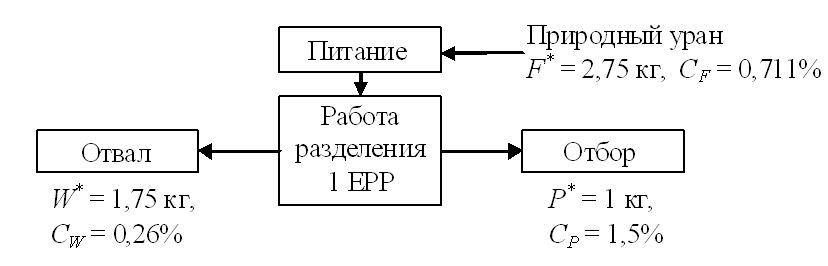
\includegraphics[scale=0.6]{img/image5.png}}
    \caption{Величины параметров разделения, соответствующие 1 ЕРР.}\label{image5}
  \end{figure}

Разделительная способность каскада обычно измеряется в ЕРР/год. При пересчете в размерность массового потока обычно используют соотношение 1 ЕРР/год = 4,69 г/с, получающееся с учетом различий в массах металлического урана и газообразного гексафторида урана.


Таким образом, в случае «слабого обогащения» на ступенях каскада могут быть сделаны общие выводы:

\noindent -- понятия <<идеальный каскад>> и <<оптимальный каскад>> идентичны;

\noindent -- результаты, следующие из теории идеального каскада и подхода Дирака и Пайерлса приводят к полезным для практики понятиям <<разделительная способность (мощность) ступени>>, <<разделительный потенциал>>, <<функция ценности>>.

\subsection{Идеальный каскад с одинаковым немалым коэффициентом разделения на ступенях.}

Если принять, что полные коэффициенты разделения ступеней $q_{s} $ каскада одинаковы и не зависят от $L_{s} $ и $\theta _{s} $, то из общего условия идеальности каскада $\alpha _{s} =\beta _{s+1} $, получающегося из \ref{GrindEQ__1_94_}, \ref{GrindEQ__1_95_} и\ref{GrindEQ__1_6_}, следует, что идеальный каскад в этом случае характеризуется двумя значениями коэффициентов разделения $\alpha _{s} ,\; \beta _{s} $, повторяющимися через ступень:

\begin{equation} \label{GrindEQ__1_132_} 
\alpha _{1} =\beta _{2} =\alpha _{3} =\beta _{4} =\; ...\; , 
\end{equation} 
\begin{equation} \label{GrindEQ__1_133_} 
\beta _{1} =\alpha _{2} =\beta _{3} =\alpha _{4} =\; .... 
\end{equation} 

Из условия идеальности $\alpha _{s} =\beta _{s+1} $ также следует, что
\begin{equation} \label{GrindEQ__1_134_} 
R_{s} =\alpha _{s-1} R_{s-1} =\frac{R_{s+1} }{\beta _{s+1} } ,                              
\end{equation} 

где   $R_{s} =\frac{c_{s} }{1-c_{s} } $.

Если расчет ведется, начиная от первой ступени каскада, то, учитывая условие \ref{GrindEQ__1_134_}, можно записать
\begin{equation} \label{GrindEQ__1_135_} 
R_{1} =R''_{1} \beta _{1} ,          
\end{equation} 

где $R''_{1} =R_{w} $ - относительная концентрация ценного изотопа в потоке отвала. Далее
\begin{equation} \label{GrindEQ__1_136_} 
R_{2} =R'_{1} =\alpha _{1} R_{1} =\alpha _{1} \beta _{1} R_{w} =R_{w} q,  
\end{equation} 
\begin{equation} \label{GrindEQ__1_137_} 
R_{3} =R'_{2} =\alpha _{2} R_{2} =\alpha _{2} qR_{w} =R_{w} q\beta _{1} ,  
\end{equation} 

\begin{equation} \label{GrindEQ__1_138_} 
    R_{4} =R'_{3} =\alpha _{3} R_{3} =\alpha _{1} \beta _{1} R_{w} q=R_{w} q^{2},  
\end{equation} 


Обобщение выражений \ref{GrindEQ__1_135_}-\ref{GrindEQ__1_138_} приводит к следующим формулам для относительных концентраций на входах в ступени идеального каскада:

нечетные ступени:
\begin{equation} \label{GrindEQ__1_139_} 
    R_{s} =R_{w} q^{\frac{s-1}{2} } \beta _{1}; 
\end{equation} 

четные ступени:
\begin{equation} \label{GrindEQ__1_140_} 
    R_{s} =R_{w} q^{\frac{s}{2} }; 
\end{equation} 

Анализ соотношений \ref{GrindEQ__1_139_}, \ref{GrindEQ__1_140_} показывает, что существует четыре типа идеального каскада, отличающихся друг от друга числом разделительных ступеней в обогатительной и обеднительной частях и, соответственно, формулами для расчета относительных концентраций $R_{p} $ и $R_{w} $:

\textbf{\textit{\underbar{тип I}}}\underbar{:} при четном $f$-1 и четном $N-f+1$
\begin{equation} \label{GrindEQ__1_141_} 
R_{p} =R_{F} q^{\frac{N-f+1}{2} } ,\, \, \, R_{w} =R_{F} q^{-\frac{f-1}{2} } \beta _{1} {}^{-1} ; 
\end{equation} 

\textbf{\textit{\underbar{тип II}}}: при четном $f$-1 и нечетном $N-f+1$
\begin{equation} \label{GrindEQ__1_142_} 
R_{p} =R_{F} q^{\frac{N-f+2}{2} } \beta _{1}^{-1} ,\, \, \, R_{w} =R_{F} q^{-\frac{f-1}{2} } \beta _{1} {}^{-1} ; 
\end{equation} 

\textbf{\textit{\underbar{тип III}}}: при нечетном $f$-1 и четном $N-f+1$
\begin{equation} \label{GrindEQ__1_143_} 
R_{p} =R_{F} q^{\frac{N-f+1}{2} } ,\, \, \, R_{w} =R_{F} q^{-\frac{f}{2} } ; 
\end{equation} 

\textbf{\textit{\underbar{тип IV}}}: при нечетном $f$-1 и нечетном $N-f+1$
\begin{equation} \label{GrindEQ__1_144_} 
R_{p} =R_{F} q^{\frac{N-f}{2} } \beta _{1} ,\, \, \, R_{w} =R_{F} q^{-\frac{f}{2} } . 
\end{equation} 

где $R_{F} ,\; R_{p} \; ,R_{w} $ - относительные концентрации ценного изотопа соответственно в потоке питания, отбора и отвала.

 Отметим, что при симметричном режиме работы первой ступени каскада, то есть при одинаковых коэффициентах разделения по обогащённой и обеднённой фракциям ($\alpha _{1} =\beta _{1} $), все ступени каскада будут работать в симметричном режиме, Другими словами $\alpha $ и $\beta $ будут одинаковы для всех ступеней каскада и равны
\begin{equation} \label{GrindEQ__1_145_} 
\alpha =\beta =\sqrt{q} .                                 
\end{equation} 

Идеальный каскад со ступенями, работающими в симметричном режиме, впервые был рассмотрен К.Коэном [1]. В этом случае относительные концентрации не зависят от соотношения числа ступеней в отборной и отвальной частях каскада и формулы \ref{GrindEQ__1_139_} - \ref{GrindEQ__1_144_} приводятся к одинаковому виду
\begin{equation} \label{GrindEQ__1_146_} 
R_{s} =R_{w} q^{\frac{s}{2} } ,                                      
\end{equation} 
\begin{equation} \label{GrindEQ__1_147_} 
R_{p} =R_{F} q^{\frac{N-f+1}{2} } ,\, \, \, R_{w} =R_{F} q^{-\frac{f}{2} } .                
\end{equation} 

Отметим, что в соответствии с соотношением \ref{GrindEQ__1_96_} величина параметра $\beta _{1} $ и коэффициента деления потока на первой ступени $\theta _{1} $ однозначно связаны. Наиболее простой вид эта связь имеет место при $c<<1$.
\begin{equation} \label{GrindEQ__1_148_} 
\theta _{1} =\frac{\beta _{1} -1}{q-1} ,                                     
\end{equation} 

и соответственно
\begin{equation} \label{GrindEQ__1_149_} 
\beta _{1} =1+\theta _{1} (q-1).                           
\end{equation} 

Как следует из \ref{GrindEQ__1_132_} и \ref{GrindEQ__1_148_}, величина $\theta _{s} $ в этом случае принимает два значения, повторяющиеся через ступень.

В общем случае анализ полученных соотношений \ref{GrindEQ__1_141_} -- \ref{GrindEQ__1_144_}, \ref{GrindEQ__1_147_} позволяет сделать следующий вывод. При заданных величинах $q,\; N,\; f$ и $c_{F} $ (III тип идеального каскада) или $q,\; N,\; f$, $c_{F} $ и $\beta _{1} $ ($\theta _{1} $) (I, II и IV типы идеального каскада) расчет каскада (нахождение распределений $L(s),\; \theta (s)\; 8\; c(s)$, включая концентрации $c_{P} $ и $c_{W} $), труда не представляет. Причем для III-го типа величины $c_{P} $ и $c_{W} $ не зависят от $\beta _{1} $, то есть в отношении выбора коэффициента деления потока $\theta _{1} $ существует произвол. При этом при варьировании $\beta _{1} $ (или $\theta _{1} $) будут меняться распределения $\beta (s)$ и $\theta (s)$, а вместе с ними и эффективность работы каждой разделительной ступени. Поэтому логично выбирать значение $\beta _{1} $($\theta _{1} $) из условия оптимальности работы ступеней идеального каскада, которое выполняется при условии минимальности относительного суммарного потока в каскаде $\sum L^{*} /P=\min  $.

Как видно из приведенной зависимости на рис.1.11 для случая \textit{с}$\mathrm{<}$$\mathrm{<}$1 минимальный суммарный поток в идеальном каскаде III-го типа, рассчитанном для следующих значений параметров: $N=9,\; f=2,\; c_{F} =0,711\% ,\; c_{P} =4,4\% ,\; c_{W} =0,45\% ,\; q=1,6$, соответствует случаю, когда он построен из симметричных ступеней, то есть $\theta _{1} =1/\left(\sqrt{q} +1\right)$.



Рис. 1.11. Зависимость относительного суммарного потока в идеальном каскаде от величины $\theta _{} $

При расчете каскадов I, II и IV типов с изменением коэффициента деления потока на первой ступени $\theta _{1} $ будет меняться не только величина суммарного потока в каскаде, но и величины концевых концентраций ($c_{W} $ - в каскаде I-го, $c_{P} $ и $c_{W} $ - в каскаде II-го и $c_{P} $ - в каскаде IV-го типа). Для этих типов идеального каскада каждому значению $\beta _{1} $($\theta _{1} $) соответствует свой идеальный каскад. Расчеты показывают, что и в этом случае из семейства всех возможных идеальных каскадов наименьший суммарный поток будет в каскаде, в котором выполняется условие $\beta _{1} =\sqrt{q} $, то есть в каскаде из симметричных элементов.

Задача расчета идеального каскада заметно усложняется в том случае, когда заданы величины $q,\; c_{P} ,\; c_{W} $ и $c_{F} $, а требуется найти кроме распределений $L(s),\; \theta (s)\; $ и $c(s)$ по ступеням каскада также общее количество ступеней \textit{N} и номер ступени\textit{ f}, в которую подают поток питания. В этом случае решение задачи следует начать с поиска типа идеального каскада, способного обеспечить в выходных потоках значения заданных концентраций $c_{P} $ и $c_{W} $. Решая систему \ref{GrindEQ__1_147_} из 2-х алгебраических уравнений при заданных значениях концентраций и величине коэффициента разделения \textit{q}, находим величины \textit{N} и \textit{f}. При целочисленных значениях \textit{N} и \textit{f} дальнейший расчет идеального каскада из симметричных ступеней труда не представляет. При дробных значениях \textit{N} и \textit{f} необходимо подобрать тот тип идеального каскада, который при соответствующем подборе целочисленных величин \textit{N} и \textit{f}, а также коэффициента деления потока $\theta _{1} $ обеспечит величины концентраций в выходных потоках, которые будут ближе всего к заданным. 

Например, для идеального каскада типа IV при \textit{q}=1,59 и $c_{F} =0,71\% ,\; \; c_{P} =4,4\% $, а также \textit{N}=9, \textit{f}=3 получены следующие значения параметров [19]. Величина концентрации ценного компонента в отвале при этом получается равной 0,44\% (см. таблицу 1.2).

В рассмотренном примере в идеальном каскаде из несимметричных разделительных элементов коэффициент деления потока и удельная разделительная способность пилообразно меняются от ступени к ступени. Нечетные ступени в каскаде имеют значения $\theta _{s} =0,118$ и $\delta U_{s} /L^{*} {}_{s} =1,48$$.$10${}^{-2}$, а четные - $\theta _{s} =0,981-0,982$ и $\delta U_{s} /L^{*} {}_{s} =1,71$$.$10${}^{-2}$. 

 Относительный суммарный поток в таком каскаде равен $\sum _{s}L_{s}^{*} /P $=299,99, а сумма относительных разделительных способностей (мощностей) всех ступеней каскада, то есть разделительная способность каскада в целом равна $\sum _{s}\delta U_{s} /P $=4,793. Среднее значение разделительной способности $\overline{\delta U_{s} /L_{s}^{*} }$ ступени составляет 1,58$.$10${}^{-2}$.


В идеальном каскаде из симметричных ступеней суммарный поток может быть рассчитан с помощью простого аналитического выражения. С учетом равенства $\alpha =\beta =\sqrt{q} $, а также формул \ref{GrindEQ__1_7_}, \ref{GrindEQ__1_9_} соотношения \ref{GrindEQ__1_107_} могут быть переписаны в виде:

\begin{equation} \label{GrindEQ__1_150_} 
\theta _{s} =\frac{1+(\alpha -1)c_{s} }{\alpha +1} ,                            
\end{equation} 
\begin{equation} \label{GrindEQ__1_151_} 
L_{s}^{*} =\frac{\alpha +1}{\alpha -1} P\frac{(c_{P} -c_{s} )}{c_{s} (1-c_{s} )}  
\end{equation} 

- для обогатительной части каскада; 
\begin{equation} \label{GrindEQ__1_152_} 
L_{s}^{*} =\frac{\alpha +1}{\alpha -1} W\frac{(c_{s} -c_{w} )}{c_{s} (1-c_{s} )}  
\end{equation} 

- для обеднительной части каскада.

Формулы \ref{GrindEQ__1_151_} и \ref{GrindEQ__1_152_} описывают дискретные распределения потоков по ступеням идеального каскада из симметричных ступеней. Величина потока на ступени с номером (\textit{s}=\textit{f}) имеет максимальное значение. В обогатительной части поток питания ступеней уменьшается в направлении отбора каскада, а в обеднительной части - в сторону отвала.

 В соответствии с формулами \ref{GrindEQ__1_141_}-\ref{GrindEQ__1_142_} относительные концентрации ценного изотопа в отборе и в отвале связаны с числом ступеней в обогатительной и обеднительной частях каскада соотношениями \ref{GrindEQ__1_147_}. Следовательно, степень разделения каскада при заданных величинах \textit{N} и \textit{f} равна:
\begin{equation} \label{GrindEQ__1_153_} 
\frac{R_{p} }{R_{w} } =\alpha ^{N+1} =q^{\frac{N+1}{2} } .                         
\end{equation} 

 В соответствии с \ref{GrindEQ__1_153_} число ступеней в идеальном каскаде при выполнении условия $\alpha =\beta $ будет равно

\begin{equation} \label{GrindEQ__1_154_} 
N =\frac{2}{\ln q} \ln \frac{R_{p} }{R_{w} } -1.
\end{equation} 

 Очевидно, что для достижения такой же степени разделения, как в безотборном режиме, в данном случае потребуется примерно вдвое больше ступеней.

 Для нахождения суммарного потока все концентрации, входящие в \ref{GrindEQ__1_151_} и \ref{GrindEQ__1_152_}, выразим через $R_{F} ,\; N$ и \textit{f} , имея в виду \ref{GrindEQ__1_146_} и \ref{GrindEQ__1_147_}, а также очевидное соотношение $R_{s} =\frac{c_{s} }{1-c_{s} } $. В результате формулы \ref{GrindEQ__1_151_} и \ref{GrindEQ__1_152_} приобретут вид:

 для обогатительной части каскада
\begin{equation} \label{GrindEQ__1_155_} 
L_{s}^{*} =\frac{\alpha +1}{\alpha -1} \frac{1}{R_{F} } Pc_{p} \left[\alpha ^{f-s} -\alpha ^{f-N-1} +R_{F} (1-\alpha ^{s-N-1} )\right];           
\end{equation} 

 для обеднительной части каскада
\begin{equation} \label{GrindEQ__1_156_} 
L_{s}^{*} =\frac{\alpha +1}{\alpha -1} \frac{1}{R_{F} } Wc_{w} \left[\alpha ^{f} -\alpha ^{f-s} +R_{F} (\alpha ^{s} -1)\right].                     
\end{equation} 

При суммировании $L_{s}^{*} $ по ступеням каскада учтем, что для любого $m\ge 0$ $\sum _{s=0}^{m}\alpha ^{s}  =\frac{\alpha ^{m+1} -1}{\alpha -1} $, а параметры $N-f+1$ и \textit{f} связаны с относительными концентрациями $R_{p} ,\; R_{F} ,$ и $R_{w} $ соотношениями \ref{GrindEQ__1_147_}. Принимая это во внимание, получим:

              для обогатительной части каскада
\begin{equation} \label{GrindEQ__1_157_} 
\sum _{s=f}^{N}L_{s}^{*}  =P\left\{\frac{\alpha +1}{\alpha -1} \frac{1}{\ln \alpha } (2c_{p} -1)\ln \frac{R_{p} }{R_{F} } +\frac{(c_{p} -c_{F} )\left[\alpha (1-c_{F} )-c_{F} \right]}{(\alpha -1)c_{F} (1-C_{F} )} \right\},~ 
\end{equation} 

              для обеднительной части каскада
\begin{equation} \label{GrindEQ__1_158_} 
\sum _{s=1}^{f-1}L_{s}^{*}  =W\left\{\frac{\alpha +1}{\alpha -1} \frac{1}{\ln \alpha } (2c_{w} -1)\ln \frac{R_{w} }{R_{F} } +\frac{(c_{w} -c_{F} )\left[\alpha (1-c_{F} )-c_{F} \right]}{(\alpha -1)c_{F} (1-C_{F} )} \right\}, 
\end{equation} 

Суммируя \ref{GrindEQ__1_157_} и \ref{GrindEQ__1_158_} с учетом \ref{GrindEQ__1_77_} и \ref{GrindEQ__1_78_}, получим
\[\sum _{s=1}^{N}L_{s}^{*}  =\frac{\alpha +1}{(\alpha -1)\ln \alpha } \left[P(2c_{p} -1)\ln \frac{c_{p} }{1-c_{p} } +W(2c_{w} -1)\ln \frac{c_{w} }{1-c_{w} } -\right. \] 
\begin{equation} \label{GrindEQ__1_159_} 
\left. -F(2c_{F} -1)\ln \frac{c_{F} }{1-c_{F} } \right].                                       
\end{equation} 

Если разделить левую и правую часть \ref{GrindEQ__1_159_} на первый множитель в правой части, то получим
\begin{equation} \label{GrindEQ__1_160_} 
\begin{array}{l} {\sum _{s=1}^{N}L_{s}^{*} \frac{(\alpha -1)\ln \alpha }{\alpha +1}  =P(2c_{p} -1)\ln \frac{c_{p} }{1-c_{p} } +W(2c_{w} -1)\ln \frac{c_{w} }{1-c_{w} } -} \\ {\; \; \; \; \; \; \; \; \; \; \; \; \; \; \; \; \; \; \; \; \; \; -F(2c_{F} -1)\ln \frac{c_{F} }{1-c_{F} } \mathrm{\; .}} \end{array} 
\end{equation} 

Правая часть выражения \ref{GrindEQ__1_160_} по форме записи соответствует полезной разделительной способности каскада, введенной в п. 1.5. В левой части \ref{GrindEQ__1_160_} под знаком суммы стоит величина, которую можно интерпретировать как разделительную способность симметричной разделительной ступени
\begin{equation} \label{GrindEQ__1_161_} 
\delta U_{s} =L_{s}^{*} \frac{(\alpha +1)\ln \alpha }{\alpha -1} .                              
\end{equation} 

Если все ступени каскада состоят из идентичных элементов, то суммарное число таких элементов $Z_{84} $ будет равно
\begin{equation} \label{GrindEQ__1_162_} 
Z_{84} =\frac{\Delta U}{L_{M} \frac{(\alpha +1)\ln \alpha }{\alpha -1} } ,                                
\end{equation} 

где  $\Delta U=PV(c_{p} )+WV(c_{w} )-FV(c_{F} )$, $L_{M} $ - поток на входе в  разделительный элемент.

 Характерно, что для всех ступеней каскада в случае, когда $\alpha =\beta $, величина удельной разделительной способности $\delta U_{s} /L_{s} $ одинакова и равна
\begin{equation} \label{GrindEQ__1_163_} 
\frac{\delta U_{s} }{L_{s}^{*} } =\frac{\alpha -1}{\alpha +1} \ln \alpha .     ~~~~~~~~~~~~~~~~~~~~~~~~~~~~~~~~~ 
\end{equation} 

Остается ответить на вопрос: является ли $Z_{84} $ в соотношении \ref{GrindEQ__1_162_} минимальной величиной при заданных значениях $P,\; c_{P} ,\; c_{W} $? Другими словами, является ли в данном случае <<идеальный каскад>> <<оптимальным каскадом>>? Используя аналитические подходы, ответить на этот вопрос невозможно.




\section{Задания для самостоятельного выполнения.}


Задания
